\documentclass[twoside]{uva-inf-bachelor-thesis}
\usepackage[english]{babel}

% Filling your thesis with only lorem ipsum is not advised.
\usepackage{lipsum}
\usepackage{float}
\usepackage{amsthm}

\usepackage{lscape}

% To allow appendixes as chapters
\usepackage[toc,page]{appendix}

\theoremstyle{definition}
\newtheorem{definition}{Definition}[section]
\newtheorem{hypothesis}{Hypothesis}

% For the ReadMe
\usepackage{markdown}

% \usepackage{cite}
\usepackage[style=authoryear-comp]{biblatex}
\addbibresource{Project/Thesis/LaTeX/main.bib}

% Title Page
\title{Development of an interactive experiment on the effect of sequential information on the formation of generic beliefs}
\author{Bodi Boelé}
\supervisors{dr. Patricia Mirabile}
\signedby{-}

\begin{document}
\maketitle

\begin{abstract}
Building on earlier (ongoing) investigations on the semantics of generics, this thesis will discuss the online implementation of a dedicated tool to host an interactive experiment and then use this tool to execute a pilot experiment focused on optimising the efficiency and user experience of the tool.

The purpose of the experiment is to investigate the claim that generics are formed about a target group through a process of associative learning, which considers both the target of the learning as well as a relevant contrast class.

The experiment described in this thesis is part of an ongoing investigation by an NWO research project on generics at the Institute for Logic, Language and Computation (ILLC) of the University of Amsterdam.
\end{abstract}

\tableofcontents

\chapter{Introduction}
\section{Generic statements}
Generic statements are sentences which are used to attribute features, patterns, sentiments and other beliefs to a group.
`Ducks lay eggs', `tigers are striped', `lions have manes' and `ticks spread Lyme disease' are examples of generic statements. Generic statements express generalisations about the members of a kind and lack any form of quantification and are therefore `bare' statements. Other than bare, there are also other types of statements that describe generalisations, such as quantified statements. Quantification's that can be found in statements are adjectives such as `most', `all' and `many', examples of the (universally) quantified form of previously mentioned examples are `all ducks lay eggs' and `all tigers are striped'. This research will focus on `bare generics' and disregard any other type of statements.

`Bare' generic statements express useful generalisations, but an unambiguous conclusion on when people think these statements are true can not be formed. There is no unique critical point of statistical prevalence of the feature in the kind where people in general tend to designate a statement as true. For example when people have to judge the statement `lions have manes', the predominant judgement will be that the statement is true, although less than 50\% of lions (only male lions will grow manes, and only from the age of two years) have manes. When asked about the statement `ticks spread Lyme disease' the predominant conclusion will as well tend to be that the sentence is true, even though the statement is only true for 2.7\% \parencite{rivm_2019} of tick bites that actually transfer the disease whereas 20\% of ticks carry the disease. \cite{leslie2011all} investigated these differences between the result that was empirically gathered through experiments and the response that was expected based on the statistical information provided to the participants. In their study, they also compare the way participants interpret a given generic with the way participants interpret the corresponding universally quantified statement. They were able to show the existence of a generic overgeneralization effect, which occurs for statements describing minority characteristics when the corresponding generic statement is also true. Thus they showed that people have the tendency to interpret the statements `ducks lay eggs' and `all ducks lay eggs' as having the same implications. The experiment this thesis is about, will try to help solve this puzzle on the difference between the theorised formal meaning of those sentences and the empirical meaning people give to those sentences.

\section{Formal and Empirical research}
There are two main types of research on generics, empirical and formal research. Where empirical research focuses on direct observations and experiences, formal research focuses on modelling and formulating formal rules and proving the correctness of a rule regarding production and interpretation of natural language. The formal approach therefore is more limited in covering all actual cases. The formal approach to generics is criticised by many because of the proposed interpretation that any formal rule should be based solely on probabilistic considerations i.e. the majority rule. Therefore rules are defined that are statistically correct, even though the researchers themselves know of the various counter-examples in natural language to the rule. This rigidity makes it impossible to take into account the mismatch between thoughts of people and the probability given.

In this project generics the two approaches are closely related and are viewed as being complementary with each other. In an ideal situation the rules formulated in formal research will be acknowledged using data gathered through empirical research.


\section{Goal}
The goal of this research project is to implement an interactive experiment. The focus of this experiment will be on the importance of the learning process on the formation of beliefs regarding generic statements. This project seeks to implement an online tool which will first be tested using a pilot experiment. As a follow up the tool will be used in an ongoing research project by \cite{RooijSchulzGenAlt} on `Generics and Alternatives`. In their research, \cite{RooijSchulzGenAlt} use a formal approach to the meaning of generic sentences. Their paper discusses three studies that tested their proposal. They presented participants with visual stimuli and asked them to judge the assertability of generic sentences describing the stimuli. In their conclusion they mention a shortcoming of their research that should be the focus of future work. The shortcoming mentioned is that the experiment did not take the into account the learning dimension that is described in the theory from \cite{RooijSchulzGenAlt}. According to their theory, the way people take the given contrast into account is a learning process, that can be modelled by the Rescorla–Wagner learning model, which conceptualises learning in terms of an association between conditioned and unconditioned stimuli \parencite{wilson_2012}. 

Ivan Pavlov started research on, what is nowadays called, Classical Conditioning in the 1890s. The model he created showed the correlation between trigger (A) and result (B), and how the influence of $A \Rightarrow B$ was related to $A \Rightarrow \neg B$. For example, Pavlov used dogs in his investigation and he found that dogs start drooling when they are offered food. Giving a signal ($A$) before giving food($B$) to the dog would let the dog associate that signal with getting food. This would eventually result in the dog starting drooling every time the signal($A$) was given, even though no food ($\neg B$) was offered \parencite{gormezano1966classical}.
The Rescorla–Wagner model, which further develops this paradigm, would for example suggest that pairing the Pavlov signal with a very tasty piece of food (e.g. a juicy steak) would have a greater likelihood of causing salivation than pairing the signal with a less tasty piece of food. 

The role of this effect on the experiment we  conducted is about the belief resulting from the information a participant has been exposed to. According to the theory people's belief in a generic at a time $t$ is the result of the number of times people have observed the association between group and feature compared to the number of times people have not observed that same association until the given time $t$. At time $t+N$, after observing new information, the belief in a generic will adapt again, depending on the content of the information received. For example, `Birds lay eggs' will be interpreted, at a given time $t$, as if it were true because people have been exposed to more information about cases where something was a bird and it laying eggs compared to cases where something was a bird and it not laying eggs. The strength of this belief will decrease if people observe a new case, at time $t+1$, where a bird does not lay eggs. To test this theory on associative learning, the experiment discussed in this thesis is an experiment on sequential learning.


\chapter{Theoretical background}
\subsection{Intuitions observed by empirical research}
Experimental psychology has highlighted a number of biases and preferences, among them the generic overgeneralization effect, the bias for people to accept a generic statement based on minority characteristics. For example people tend to classify `Men attack people' as false and `Sharks attack people' as true, even though the chance of men attacking people is vastly higher than the chance of sharks attacking people. This `negative' bias towards sharks, and non-human entities in general, is firstly caused by the striking type of the used predicate. Secondly people are more negatively biased towards non-human categories, as has been indicated in experiments conducted by \cite{tasimi2017differences}. In different experiments participants were assigned a domain, either people or tools and things. They were then given a statement about one of these domains and had to rate the chosen domain as helpful or dangerous. This experiment showed a preference where people tend to be more negative towards generics describing non-human entities. 
The overarching research project of this thesis is about the formation of generic beliefs. In the experiment this thesis is about, participants are shown different images. In case the experiment would incorporate images showing different domains of entities (e.g. human entities) then such a bias towards certain entities could influence how a statement is rated and therefore it is important to acknowledge the possibility of such biases during the experiment.

A bare generic statement, such as `ducks lay eggs,' appears to be true, since many ducks lay eggs. The universally quantified version of this generic statement, `All ducks lay eggs', should on the other hand be rejected by it's incorrectness, because it is physically impossible for male ducks to lay eggs. Different experiments showed that this statement is interpreted as true, even though it only correctly describes 50\% of the cases. The paper by \cite{leslie2011all} set out different experiments focusing on this phenomena. In one of their experiments they found that, despite knowing the relevant information on a statement that lead to the adoption of a generic statement, universally quantified statements would often be inferred to be true on the basis of the generic statement. For example, after they were given information on the percentage of ducks that lay eggs, participants would still choose to classify `all ducks lay eggs' as true. In another experiment they offered the participant a correct alternative statement to the bare generic statement. For example, the participant was offered the choice between: `female ducks lay eggs' and `all ducks lay eggs' and even then the participants would hold on to the overgeneralised statement. Their research shows that people tend to falsely accept (over)generalised statements when offered a more descriptive alternative, as described in the previous section. 


\subsection{Formal research}
The initial approach to the formal analysis of generic sentences is the use of the majority rule. Assuming a sentence `tigers are striped' (form: `Gs are f') the majority rule for a generic sentence is defined as:
\theoremstyle{definition}
\begin{definition}{Majority rule}\label{def:mayjorityrule}
A generic sentence of the form `Gs are f' is true i.f.f. $P(f|G) > \frac{1}{2}$
\end{definition}
The majority rule has various shortcomings, such as the `ticks' example mentioned in the introduction. With 2.7\% this statement should come back as false, by definition of the majority rule, but somehow participants chose otherwise. In their paper \cite{RooijSchulzGenAlt} suggest that the reason for the mismatch between the majority rule's predictions and people's intuitions that they were only looking at majority rules and not taking taking into account various notions of alternatives, many shortcomings of the majority rule can be overcome, by compensating for different factors.

\cite{van2020generics} based their analysis of generic statements on the majority rule, which they borrow from the definition in \cite{cohen1996think}, on an analysis in terms of typicality. In their paper they analysed the intuition about the majority rule (Definition \ref{def:mayjorityrule}) that some authors saw to be a natural approach to formalise generic statements. Just like many, they doubt the correctness of the rule, partly due to the vagueness and context-dependence of generics. For example, they mention that in many cases people tend to accept and interpret generics based on a distorted picture of the generic statement, such as stereotyping. This is caused by the fact that during their lifetime (i.e. learning process) people are exposed to information provided by (e.g. (social) media) instead of the actual frequencies of cues.


\subsection{Role of generic beliefs}
Experimental evidence that whether a generic statement is true does not straightforwardly depends on underlying statistical prevalence of a feature among the described group dates back to as early as 1966 by \cite{gilson1965subjective}. According to \cite{cimpian2010generic} `generic statements require little evidence for acceptance' such as the previously mentioned tick example and other striking generics like `Rottweilers maul children' and `Lions eat people' who appear as true, even though these statements are only true for exceptional cases. According to their research generic statements are often judged as true based on little evidence. Using the `ticks spread Lyme disease' example, people tend to believe that all ticks spread Lyme disease and therefore people tend to be more afraid of ticks than you would expect from a statistical point of view. Another example is the fear of Rottweilers or the assumption that flying as a means of transport is unsafe. As suggested by \cite{van2020generics} these stereotypical assumptions are partially caused by the influence of media. Striking news, for example, gets more attention and is therefore becoming the way news media make headlines and draw attention to their media websites. Due to the extra attention and the way social media aid spreading these kinds of `trending' articles, an imbalance can occur in the way people gather information. Along with the way social media use user data to fill the user's social media feed with items that interest the user, the interest of a user in a particular matter can influence the information the user gets and therefore expose him to a distorted picture about the subject of interest. Because in those cases, the information the user receives is mostly one-sidedly in favour of a given generalisation and this can influence how people interpret generics. People base their judgement on the experience they have received instead of the entire body of existing data. This shows that the little evidence that is needed for a statement to be seen as true has far-reaching consequences (e.g. people being afraid of Rottweilers). This underlines the importance of the overarching research on how people form generic beliefs and what the effect of sequential information is on their judgement.

\section{Hypothesis}
\cite{RooijSchulzGenAlt} seeks to test two hypotheses using the tool in this thesis, which was what guided the design of the experiment. 
\begin{hypothesis}
When information is received sequentially the pattern of responses will match the pattern observed in experiments where the information is received simultaneously.
\end{hypothesis}
\begin{hypothesis}
The pattern of responses will be the pattern predicted based on the relative difference of a feature. Assertability is higher when $P(f|G) > P(f|Alt(G))$ defined in the paper by \cite{RooijSchulzGenAlt} as $$\textrm{Assertability of G's are f'} = P(f|G) - P(f|\cup \textrm{Alt}(G))$$.
\end{hypothesis}

\chapter{Methods}
\section{Experimental Setup}
This experiment builds on the basis created by \cite{RooijSchulzGenAlt}. In their experiment they show the participant a grid consisting of 2 differently coloured animals, as shown in \ref{fig:beetle_example}. The participant is asked to rate the generic statement using a continuous scale.
\begin{figure}[h]
    \centering
    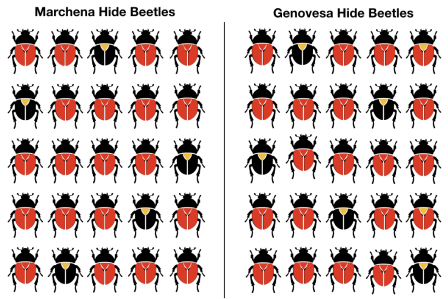
\includegraphics[width=0.7\textwidth]{Project/Thesis/LaTeX/images/beetles_example.png}
    \caption{Sample of experiments done by \cite{RooijSchulzGenAlt} as seen by the participant}
    \label{fig:beetle_example}
\end{figure}
To be able to investigate the influence of sequential data on the formation of generic beliefs, initially an experiment was set up similar as the experiment shown in \ref{fig:beetle_example}. The interactive implementation has a similar appearance, except that the field is initialised as a board consisting of tiles, somewhat resembling a game of memory. The participant must interact with the interface and sequentially (in random order) turn around all tiles, one by one. The participant will switch turns with the computer, turning around one tile at a time on their own side of the board. After all tiles have been uncovered, the participant is asked to rate a statement describing the animals from the participants side of the grid on a 7-point Likert scale. The stimuli are composed of two groups, that vary by one salient feature. These groups are shown in a non particular order, to exclude the chance of a bias from participants for a certain feature. An example of the initialised board is given in \ref{fig:example_initiated_game}.

\begin{figure}[h]
    \centering
    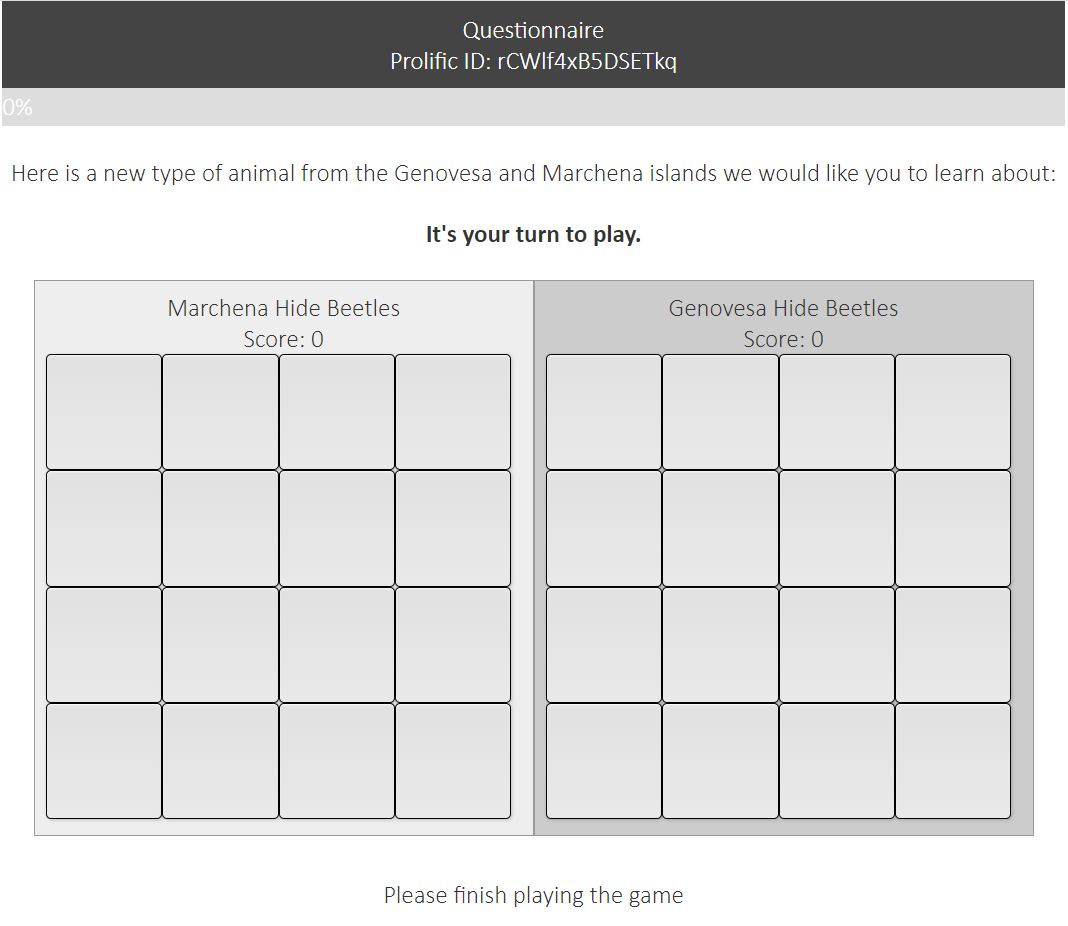
\includegraphics[width=0.7\textwidth]{Project/Thesis/LaTeX/images/uva_gen_example1.JPG}
    \caption{Sample of the experiments initial set-up}
    \label{fig:example_initiated_game}
\end{figure}
The experiment allows the participant to have a sequential learning process. By only allowing the participant to see the current information, participants follow a certain randomised timeline to complete their game. This is achieved by closing tiles after they have been uncovered. A second way to prevent learning from becoming statistical analysis, is by shifting the participant's focus. The experiment achieves this by turning the learning process into a game against a computer opponent, thus shifting the participants focus.

\section{Implementation}
The tool is created as a web based tool, which can be accessed from any non-phone device. This implementation choice was made to prevent participants from getting distracted while taking the survey. Initially Python was one of the languages of choice, but because of the focus on interaction with the tool, Python was ruled out after about a week. The tool has been written using the following web-development languages: AJAX, CSS, HTML, JavaScript, jQuery, PHP and SQL. 

The tool was developed particularly for this experiment, but has features to allow modification by a user with administrator rights. The size of the board can be changed or even randomised on a given horizontal and vertical range. The length of the experiment can also be varied, but not randomised. This allows the researcher to influence the time it takes to complete the experiment, (e.g. by increasing the board size and reducing the number of questions, the time the experiment takes can remain approximately the same).

\subsection{Participant experience}
After opening the tool in their web browser the participant will be prompted to one of two pages. If a participant does not join through a particular link, they will be direct to a thank you page, with a small description of the study.
If the participant does join through the correct link the participant is referred to the welcoming page, showing a welcome note and a button to start the questionnaire introduction. After clicking the button the participant is given information about the terms of the research and is asked for their informed consent and asked to check their prolific ID. During these first 3 pages, Google's `reCAPTCHA v3' judges if the participant is not a robot, before allowing the participant to continue. If `reCAPTCHA v3' allows the user to continue, the introduction to the study itself is shown.

The next page that the participant sees is the introduction to the experiment, after which they are lead to an instruction page. On this page the participant can become familiar with the game-like setting used in the experiment. After completing these steps, the participant is referred to a last page before they are finally able to start the experiment. This last page asks the participant to enlarge their screen and to take the survey in a calm environment.

\begin{figure}[h]
    \centering
    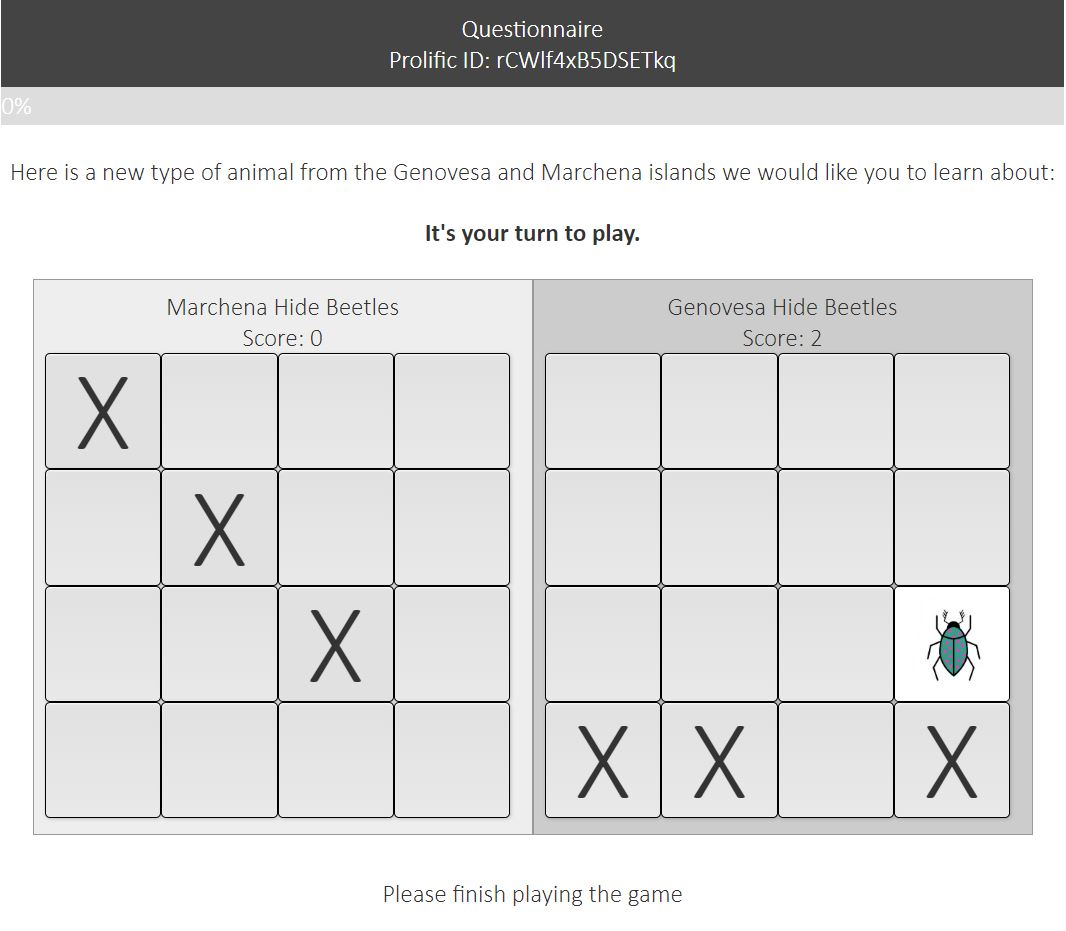
\includegraphics[width=0.7\textwidth]{Project/Thesis/LaTeX/images/uva_gen_example2.JPG}
    \caption{Sample of an ongoing experiment. Player has to match the symbol currently visible on the opponent's side.}
    \label{fig:example_ongoing_game}
\end{figure}

\subsection{Interaction with the tool}
The experiment as it was conducted is set up as two grids of 4 by 4 tiles each. The player (on the left side) plays against an opponent (randomised turns by a computer on the right side). By clicking on a tile, the participant can interact with the tool and discover the features of the group they are asked to learn about. The opponent will then turn a tile and try to find a matching card. After each counter move, the tiles are visible for a short time to show whether the tiles match, before both cards disappear again. Then the opponent is again able to select a card and the player is then able to try to match the computer's card again, as figure \ref{fig:example_ongoing_game} shows. This continues until all cards have been discovered. Then the participant will be shown a generic statement which the participant must rate on preset scale. For the experiment the preset scale is a 7-point Likert scale with values ranging from `Strongly disagree' to `Strongly agree', with this scale the board is similar to the board shown in figure \ref{fig:example_finished_game}.

\begin{figure}[h]
    \centering
    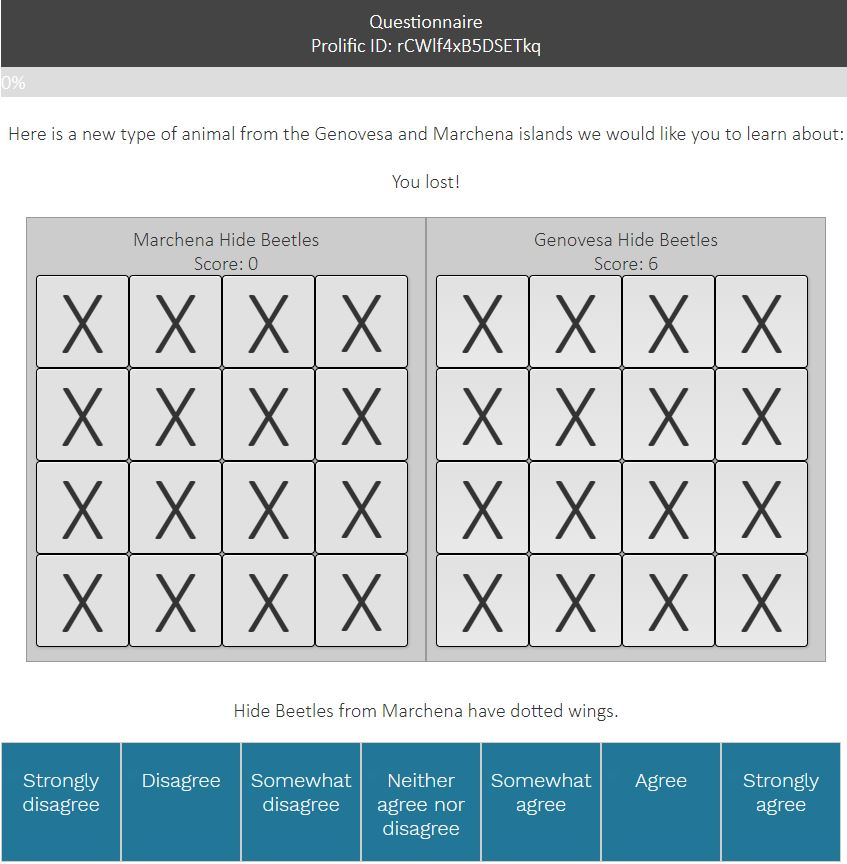
\includegraphics[width=0.7\textwidth]{Project/Thesis/LaTeX/images/uva_gen_example3.JPG}
    \caption{Completed game, waiting for user to rate the statement.}
    \label{fig:example_finished_game}
\end{figure}

\section{Data collection plan}
Data for this thesis is collected in a pilot experiment using an interactive web questionnaire created for this purpose. Participants for this pilot experiment are recruited using social (media) connections, to also be able to receive feedback on the questionnaire itself. These participants receive a link to a google form either in Dutch or in English. The form shortly introduces the goal of the experiment and asks the participant to evaluate the experiment after completing it.

The extended experiment will recruit participants via Prolific.ac, an online platform aimed
at connecting researchers and participants willing to fill in surveys and questionnaires in exchange for compensation for their time \cite{PALAN201822}.

\chapter{Results}
A pilot experiment was run on a small unrepresentative sample that allowed us to verify the usability of the design but had too low statistical power to allow us to draw any inferences regarding the empirical predictions. 

Changes have been made using their helpful feedback. For example, the first three participants all mentioned that the experiment took too long, especially the waiting for the opponent (computer) to make its turn was mentioned to be a downside. After changing the timing participants did not mention the slowness of the opponent anymore, which was helpful feedback on the improvement of the experiment.

\textbf{*Data collection is still in process, this section will be extended upon further data collection.}

\chapter{Discussion}
\section{Process}
\subsection{Setting up}
The goal of the tool is to encourage participants to sequentially learn something about the appearance of the items of a group and to apply these findings to a generic statement, which they then should rate. During the implementation and comparison to the previous experiment, some shortcomings were raised. For example the scale of the previous experiment was too precise, which can cause fluctuation in the results. Throughout the process of implementing the tool, the expected functionalities of the tool have changed quite a bit. 
\subsection{Python}
The first week the focus was on implementing the tool through Python, while this became rather difficult after going further into detail on what the tool must be capable of doing. Therefore the switch was made to using web development languages as mentioned in the implementation section. 
\subsection{Webtool}
The initial tool was going to look like a game of memory where the user had the possibility to uncover any tile one-by-one, until being shown the full grid. Mid-April Robert van Rooij, the lead researcher on the project, attended one of the weekly meetings and a number of changes was discussed to the design and implementation of the tool. Among them were the introduction of a computer player, varying the size of the grid and to interrupt the flow of clicking of the user so that the participant does not focus directly on the numerical quantity of items that present the feature of interest. After implementation of those changes, the tool was ready to be optimised using a pilot experiment midway through May.
\subsection{Late changes}
That same week, mid-May, Katrin Schulz, senior researcher on the project, provided additional feedback during a meeting. This prompted further changes on the design of the experiment and with that on the implementation of the tool. Those were changes such as letting the user experience the tool more like a game of memory, not showing the participant the tiles that had already been uncovered, letting participants try to match the card the opponent just uncovered and by keeping score of the matches that have been made by both players. The `behaviour'of the computer also needed tuning, in order for the game to be more perceived as a back and forth between the player's turns and the computer's turns. These late changes to the experimental design made the process of finalising the project less structured and limited the time for the pilot experiment to be executed. Therefore the number of participants in the pilot experiment was very limited. 
\subsection{Future work}
During future work, similar situations could be prevented by initiating the project with a meeting with all actors involved which could help to better outline the project and specifically the objective, which in this case was the way the tool was implemented. Other improvements would be, better defining a timeline, with enough space to accommodate changes.


\section{Usability}
The users so far have been more and more positive in their feedback about the tool. The tool has multiple variables that can be changed, this way the tool can be set up for multiple experiments in different ways, while maintaining the focus on testing the role of sequential information on learning. This means the tool could be adapted by the researcher to focus the experiment and gather more relevant data, but could also be adapted by other researchers to be used in an own experiment. 

From the first few results, came a complaint about using the tool as a game. The goal set for the participants is to win as much points as possible and to beat the computer by making more matches than the computer. From the participants' point of view this seems unfair, since a participant has no way of knowing which symbol is under which tile. Therefore the participant has no influence on their own score, which means winning or losing the game is based on pure luck. This could demotivate participants and make them pay less attention to the information shown to them even though there is no reward structure for winning and/or losing, which means the stakes of winning are low. From the experiment's point of view this was done on purpose. The game is only used as a cover, because showing all tiles in advance would allow them to learn all the information simultaneously instead of sequentially and in that case the tool would not be valid towards the goal of the experiment. These conflicting needs between fairness and experiment goals could be a limitation of this experimental set-up.

\section{Ethical aspects}
This thesis and the tool that has been developed takes into account various ethical aspects, such as fully informing the participants. This is done by shortly introducing the subject on the first page: `In this survey you will be asked to judge whether a sentence can be correctly asserted in a given scenario'. Further, during the survey, people get more information regarding the survey and how it works. Also participants are asked to give (written) permission for data collection by accepting the terms written in the consent form. This was done to follow ethical recommendations issued by ethics boards about conducting experiments with human beings, which requires to make sure that participants are willing to let the researcher store and process the data they generated. As defined by the declaration of Helsinki, the interest of the participant is paramount, therefore the participant also has the option to stop at any time. The confidentiality of this investigation is ensured by the fact that personal data is not stored and therefore cannot be linked to a participant. The last ethical aspect that has been covered by the tool is the debriefing. After submitting their responses, participants have the ability to read about the how and why of the research and if necessary they can even go into further detail using the provided literature references and by contacting the lead investigator. The tool itself meets certain ethical aspects, by taking a lot of care to commenting the source code in a clear way and by making the source code publicly available. This makes the experiment reproducible and at the same time allows other researchers to see how the experiment was set up. Also taking a lot of care to write a clear ReadMe file, will help towards fully informing interested parties on how to use the tool and what it was designed for.

\chapter{Conclusions}
The online implementation of a dedicated tool to host an interactive experiment and the use of this tool to execute a pilot experiment focused on optimising the efficiency and user experience of the tool and corresponding literature have been discussed in this thesis. The use of a formal approach to the meaning of generic sentences has been discussed. The shortcomings of the experiments by \cite{RooijSchulzGenAlt} were what guided the design behind this online interactive tool. According to the theory proposed in that paper, people's generalisations result from a learning process similar to that of the Rescorla-Wagner learning model, which conceptualises learning as resulting from the contrast between conditioned and unconditioned stimuli. 

The goal of this thesis was to design a tool that could be used to verify both hypotheses;
\begin{enumerate}
  \item When information is received sequentially the pattern of responses will match the pattern observed in experiments where the information is received simultaneously.
  \item The pattern of responses will be the pattern predicted based on the relative difference of a feature. Assertability is higher when $P(f|G) > P(f|Alt(G))$.
\end{enumerate}

The tool was able to capture the data needed for analysis. Unfortunately, there was not enough time available to gather enough data to do quantitative analysis on. This tool is an alternative to conventional surveying software which did not have the capability of executing the tasks that were needed for this experiment. 

Even though this thesis did not verify any hypothesis due to the limited sample size of the pilot experiment, using the feedback given throughout the pilot, the tool has been adjusted and improved accordingly, therefore the expectation is that the implementation of the tool will work as planned. 

Future work will focus on collecting enough data using the tool, to be able to verify the hypothesis of this thesis as also defined by \cite{RooijSchulzGenAlt}. 

\printbibliography
\addcontentsline{toc}{chapter}{Bibliography}

% ========================== APPENDIX ====================
\begin{appendices}
\chapter{ReadMe}
\begin{figure}[H]
    \centering
    \href{https://github.com/BodiB/UvA_Generics/blob/master/README.md}
    {
    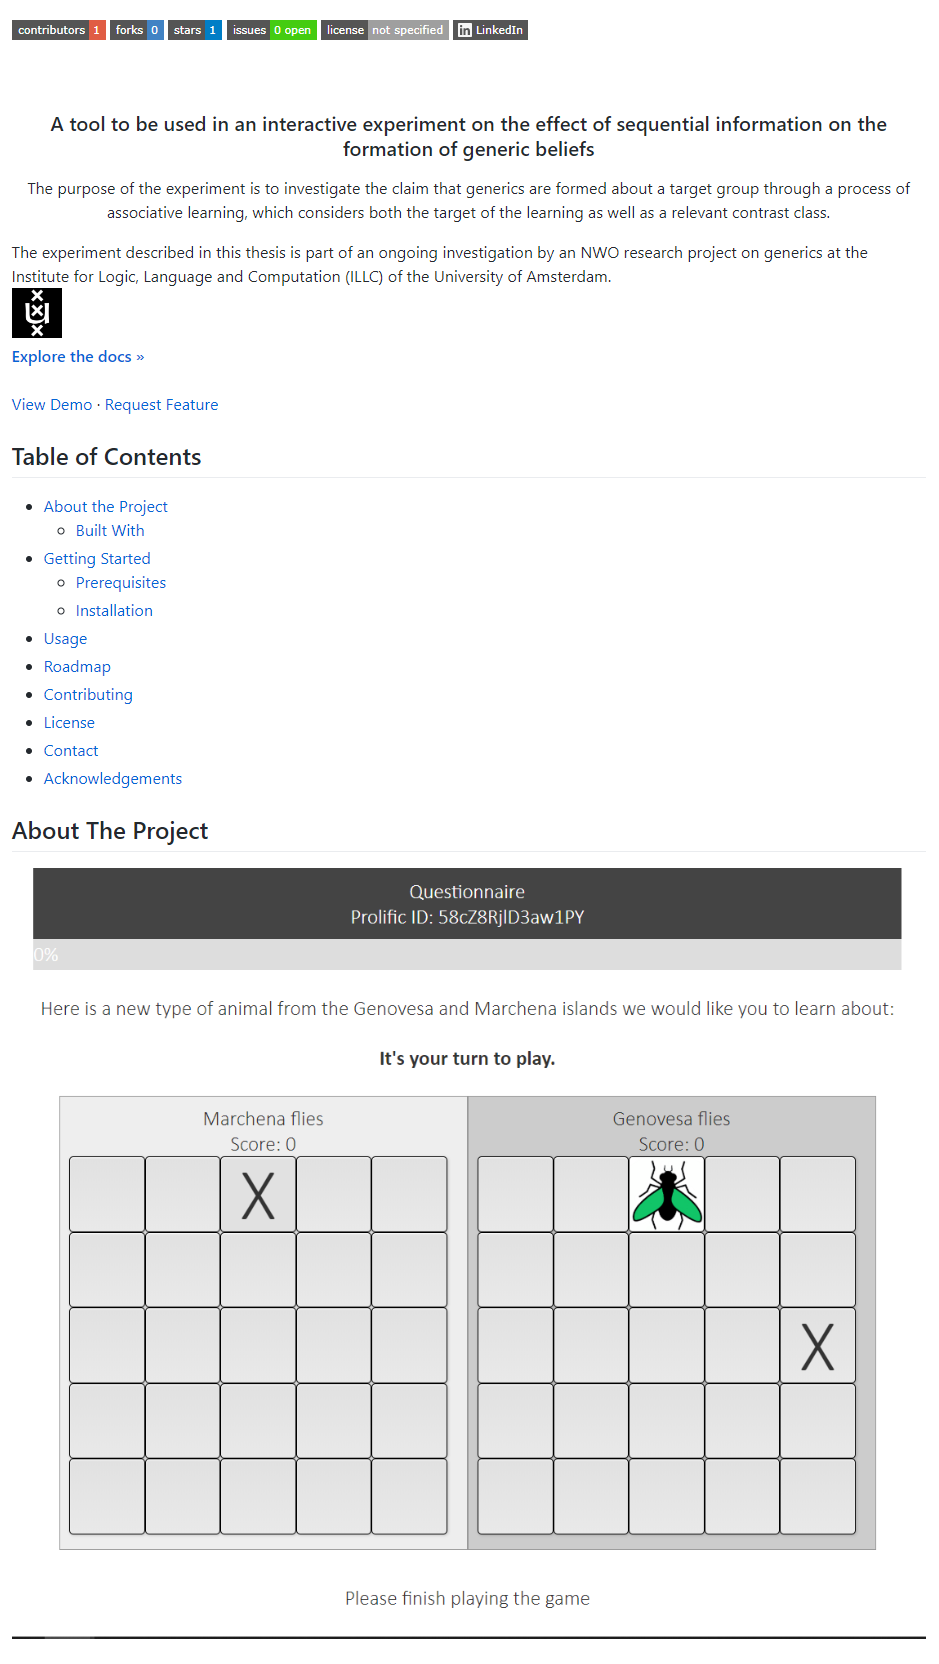
\includegraphics[width=0.55\textwidth]{Project/Thesis/LaTeX/images/ReadMe.png}
    }
    \caption{
    \href{https://github.com/BodiB/UvA_Generics/blob/master/README.md}{Sample of what the ReadMe file looks like. The entire ReadMe file can be found here https://github.com/BodiB/UvA\_Generics/blob/master/README.md}}
    \label{fig:ReadMeExample}
\end{figure}

% ReadMe AS CODE

\markdownInput{ReadMe.md}

% ReadMe AS CODE

\chapter{Form results}
\section{Dutch form response}
\href{https://docs.google.com/spreadsheets/d/1PLSfR_wIK-oo5AGtuL2LPdUuQAfAn5_-anSjShhfN1k/edit?usp=sharing}{The results gathered through the dutch form can be found on Google Docs}\\
Link (the text above is a hyperlink):\\ `https://docs.google.com/spreadsheets/d/1PLSfR\_wIK-oo5AGtuL2LPdUuQ\\AfAn5\_-anSjShhfN1k/edit?usp=sharing'
\section{English form response}
\href{https://docs.google.com/spreadsheets/d/1GP28ru4fdBwNUb0sQuQf_VmA-vZmnl0hx7HvkwK254g/edit?usp=sharing}{The results gathered through the english form can be found on Google Docs}\\
Link (the text above is a hyperlink):\\ `https://docs.google.com/spreadsheets/d/1GP28ru4fdBwNUb0sQuQf\_VmA-\\vZmnl0hx7HvkwK254g/edit?usp=sharing'
\end{appendices}

\end{document}
